%%%%%%%%%%%%%%%%%%%%%%%%%%%%%%%%%%%%%%%
%%   Nome: Leandro do Nascimento     %%
%%   Data: 10/11/2019                %%
%%   Estágio na GreenBras            %%
%%%%%%%%%%%%%%%%%%%%%%%%%%%%%%%%%%%%%%%

%define o tipo de documento: {article}, {book}, etc
\documentclass{article}

%define as margens da página
\usepackage[top=10cm,left=3cm,right=2cm,bottom=3cm]{geometry}


%\pagenumbering{arabic}
%\setcounter{page}{1}
%\pagestyle{headings}

%Declara as bibliotecas que serão utilizadas no código
\usepackage[utf8]{inputenc}
\usepackage[utf8]{inputenc}  
\usepackage[brazil]{babel}
\usepackage{fullpage}
\usepackage{parskip}
\usepackage{tikz}
\usepackage{amsmath}
\usepackage{hyperref}
\usepackage{float}
\usepackage{placeins}
\usepackage{colortbl}
\usepackage{indentfirst}
\usepackage{amsmath}
\usepackage{amssymb}
\usepackage{graphicx}
\usepackage{placeins}
\usepackage{multirow}
\usepackage{graphics}
\usepackage{caption}
\usepackage{array}
\usepackage[alf]{abntex2cite}

\linespread{1.2}

%%Declara o Título, Autor e a data do documento
%\title{Empreendedorismo social}
%\author{Jessica de Lima Brito}
%\date{10 abril de 1900}

%%Inicia documento
\begin{document}
\thispagestyle{empty} %Este comando tira numeração de página

%Título doa carta

%%%%%%%%%%%%%%%%%%%%%%%%%%%%%%%%%%%%%%%%%%%%%%%%%%%%%%%%%%
\begin{center}
\textbf{\Large{Normas para desenhos tecnicos elétricos}}    
\end{center}

\vspace{0.5cm}

\section{Normas}

™$\bullet$ \hspace{0.1cm} \textbf{NBR 10068/87} - Folhas de desenho, layout e dimensões {\color{blue}\cite{NBR10068:1987}};\\
™$\bullet$ \hspace{0.1cm} \textbf{NBR 10582/1988} - Apresentação da folha para desenho técnico {\color{blue}\cite{NBR10582:1988}};\\
™$\bullet$ \hspace{0.1cm} \textbf{NBR 13142} - Dobramento da folha {\color{blue}\cite{NBR13142:1999}}.\\

\begin{figure} [H] %[!h]
\centering
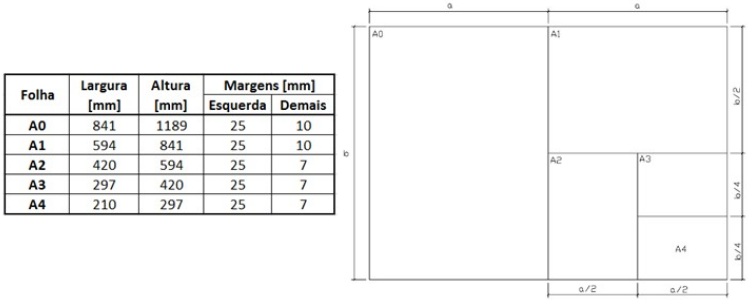
\includegraphics[scale=0.65]{Fig/Figura_DimensoesDoPapel.png} 
\caption{Dimensões do papel}
\label{fig_DimensPapel}
\end{figure}

\section{Estrutura da folha de desenho}

\hspace{1cm} A Figura \ref{fig_RegiosFolhaDesenho} mostra as diversas partes de uma folha de desenho e seus detalhes. É possível observar que as regiões acima e ao lado da etiqueta são reservadas para anotações ded revisões, observações, carimbos, etc.

\begin{figure} [H] %[!h]
\centering
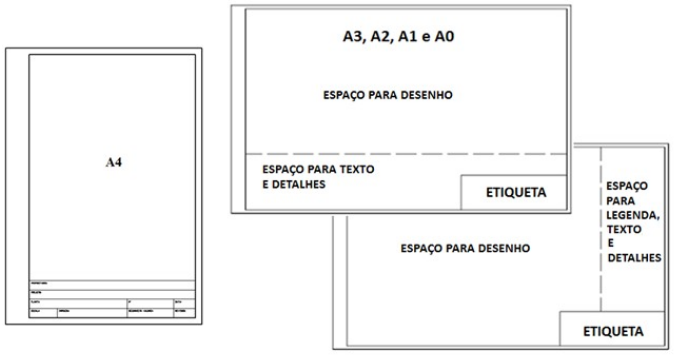
\includegraphics[scale=0.65]{Fig/Figura_RegioesFolhaDesenho.png} 
\caption{Regiões de uma folha de desenho}
\label{fig_RegiosFolhaDesenho}
\end{figure}

\section{Posição do texto no papel}

\hspace{1cm} Todos os textos escritos no pael são escritos de uma forma que possam ser lidos na base ou na direita da folha de papel, corforme ilustra a Figura \ref{fig_PosicaoTexto}.

\begin{figure} [H] %[!h]
\centering
    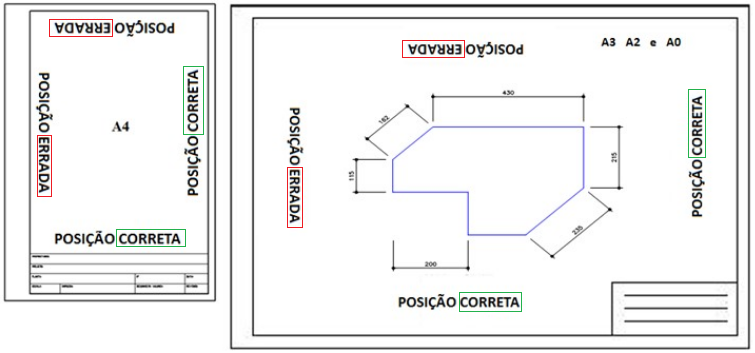
\includegraphics[scale=0.7]{Fig/Figura_PosicaoTexto.png} 
\caption{Posição do texto na folha de papel}
\label{fig_PosicaoTexto}
\end{figure}

\section{Dobragem do papel}

\hspace{1cm} A norma NBR 13142 recomenda que as cópas sejam dobradas de forma que estas fiquem similaras a uma folha A4, com espaço à esquerda de 25mm, suficiente para poder serem arquivadas em pastas. As Figuras \ref{fig_DobragemDaFolhaA3}, \ref{fig_DobragemDaFolhaA2}, \ref{fig_DobragemDaFolhaA1} e \ref{fig_DobragemDaFolhaA0} mostram a forma de dobragem das folhas nos formatos A3, A2, A1 e A0, respectivamente. 

\begin{figure} [H] %[!h]
\centering
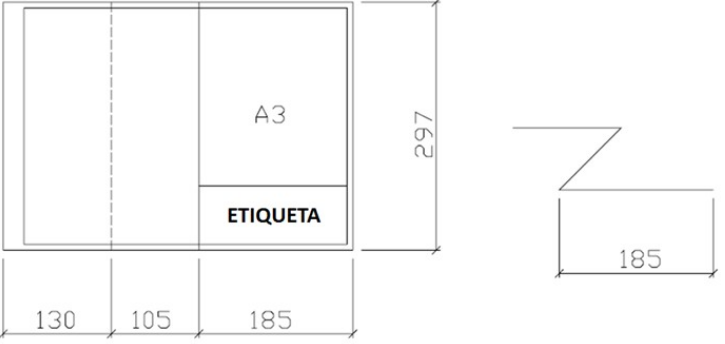
\includegraphics[scale=0.8]{Fig/Figura_DobragemFolhaA3.png} 
\caption{Dobragem da folha A3}
\label{fig_DobragemDaFolhaA3}
\end{figure}

\begin{figure} [H] %[!h]
\centering
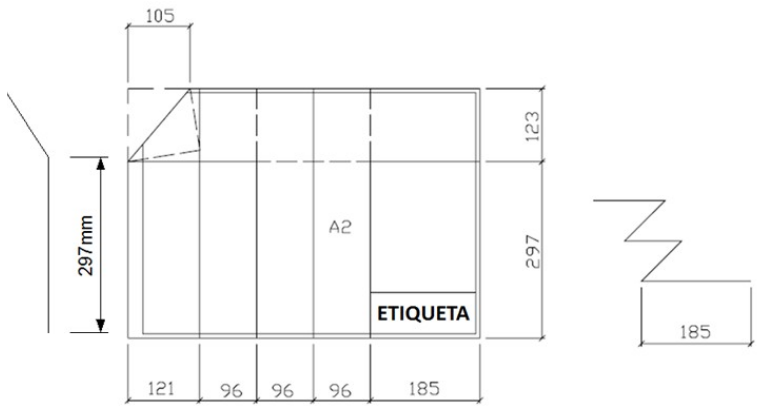
\includegraphics[scale=0.8]{Fig/Figura_DobragemFolhaA2.png} 
\caption{Dobragem da folha A2}
\label{fig_DobragemDaFolhaA2}
\end{figure}

\begin{figure} [H] %[!h]
\centering
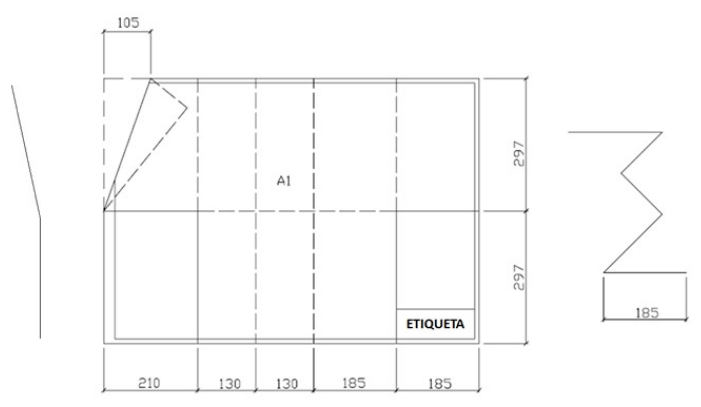
\includegraphics[scale=0.8]{Fig/Figura_DobragemFolhaA1.png} 
\caption{Dobragem da folha A1}
\label{fig_DobragemDaFolhaA1}
\end{figure}

\begin{figure} [H] %[!h]
\centering
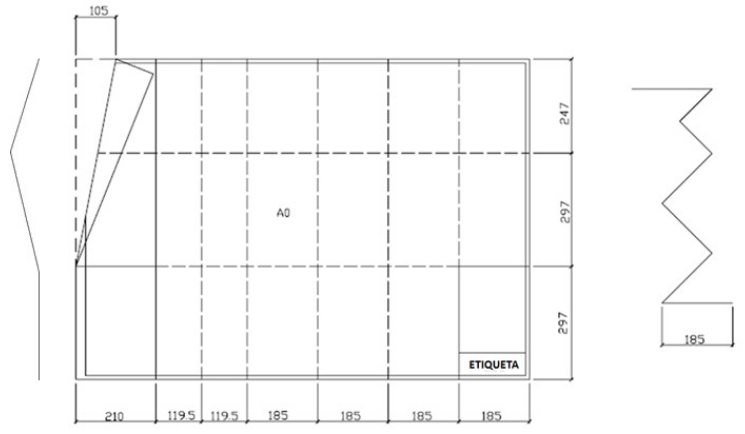
\includegraphics[scale=0.8]{Fig/Figura_DobragemFolhaA0.png} 
\caption{Dobragem da folha A0}
\label{fig_DobragemDaFolhaA0}
\end{figure}

\section{Etiqueta ou carimbo}

\hspace{1cm} O canto inferior direito das folhas de desenho deve ser reservado ao carimbo destinado à etiqueta de titulação e numeração dos desenhos. Na etiqueta devem constar, no mínimo, as seguintes informações:\\[0.3cm]
\textbf{a)} identificação da empresa e do profissional responsável pelo projeto;\\
\textbf{b)} identificação do cliente, nome do projeto ou do empreendimento;\\
\textbf{c)} título do desenho;\\
\textbf{d)} escalas;\\
\textbf{e)} data;\\
\textbf{f)} autoria do desenho e do projeto;\\
\textbf{g)} indicação de revisão.\\

(Obs.: outras informações que também devem localizar-ses próximo ao carimbo são: planta-chave; escalas gráficas; convenções gráficas; notas gerais; desenhos de referência).\\

\hspace{1cm} A Figura \ref{fig_MargensEtiquetaA4} mostra margens e etiqueta em uma folha A4. Já a Figura \ref{fig_ModeloEtiquetaA4ateA0} ilustra a um modelo de etiqueta a ser utilizada em todos os tamanhos de papeis, de A4 até A0.

\begin{figure} [H] %[!h]
\centering
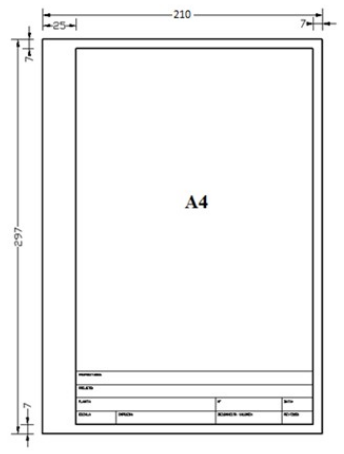
\includegraphics[scale=1.1]{Fig/Figura_MargensEtiquetaA4.png} 
\caption{Margens e etiqueta de uma folha A4}
\label{fig_MargensEtiquetaA4}
\end{figure}

\begin{figure} [H] %[!h]
\centering
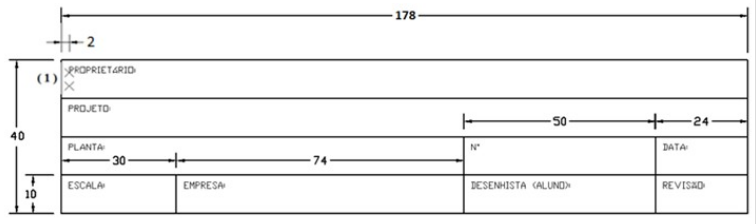
\includegraphics[scale=0.8]{Fig/Figura_ModeloEtiquetaA4ateA0.png} 
\caption{Modelo de etiqueta utilizado em A4, A3, A2 e A0}
\label{fig_ModeloEtiquetaA4ateA0}
\end{figure}
    
\hspace{1cm} A Figura \ref{fig_ExemploEtiquetaOuCarimbo} traz outro exemplo de etiqueta ou carimbo.

\begin{figure} [H] %[!h]
\centering
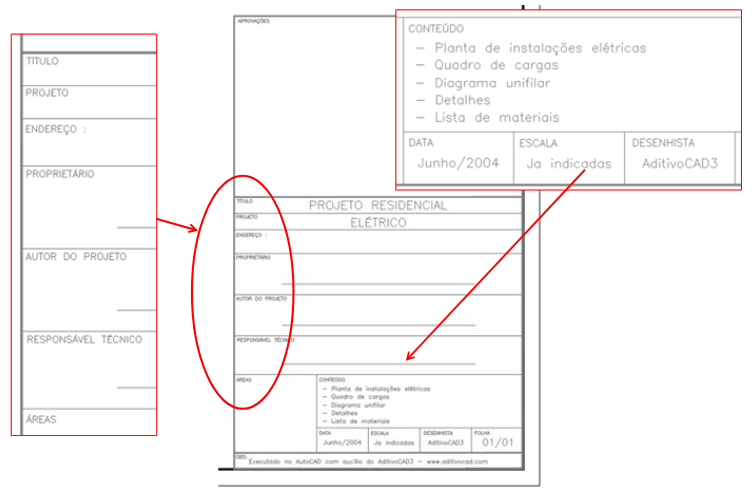
\includegraphics[scale=0.8]{Fig/Figura_ExemploEtiquetaOuCarimbo.png} 
\caption{Exemplo de etiqueta ou carimbo}
\label{fig_ExemploEtiquetaOuCarimbo}
\end{figure}

\section{Numeração de folhas}

\hspace{1cm} Junto com o número da folha usualmente se informa o total de folhas do projeto. Ex.: 2/9 significa; folha 2 de um total de 9 folhas. Uma nomeração de folha é mostrada na Figura \ref{fig_NumeracaoFolhas}.

\begin{figure} [H] %[!h]
\centering
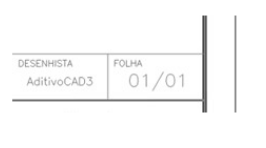
\includegraphics[scale=0.8]{Fig/Figura_ExemploNumeracaoPagina.png} 
\caption{Exemplo de numeração de folha}
\label{fig_NumeracaoFolhas}
\end{figure}

\section{Marcas de revisão}

\hspace{1cm} Conforme a NBR 10582, a tábua de revisão é utilizada para registrar correções, alterações ou acréscimos feitos no desenho. Busca registrar com clareza as infiormações referentes ao que foi alterado de uma versão do desenho para outra. Deve conter segundo a referida norma:\\
™$\bullet$ \hspace{0.1cm} Designação da revisão;\\
™$\bullet$ \hspace{0.1cm} Número do lugar onde a correção foi feita;\\
™$\bullet$ \hspace{0.1cm} Informação do assunto da revisão;\\
™$\bullet$ \hspace{0.1cm} Assinatura do responsável da revisão\\
™$\bullet$ \hspace{0.1cm} Data da revisão.\\

\begin{figure} [H] %[!h]
\centering
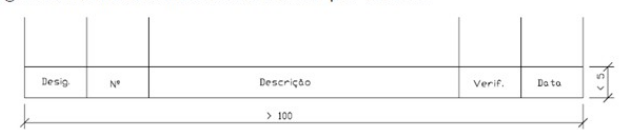
\includegraphics[scale=1]{Fig/Figura_MarcasDeRevisao.png} 
\caption{Marca de revisão}
\label{fig_MarcaDeRevisao}
\end{figure}

\section{Legenda}

\hspace{1cm} A legenda ilustrada na Figura \ref{fig_ExemploLegenda} é uma tabela contendo na coluna da direita os símbolos utilizados no projeto elétrico e na coluna da esquerda uma descrição resumida (mas completa) do material elétrico a ser instalado na obra.

\begin{figure} [H] %[!h]
\centering
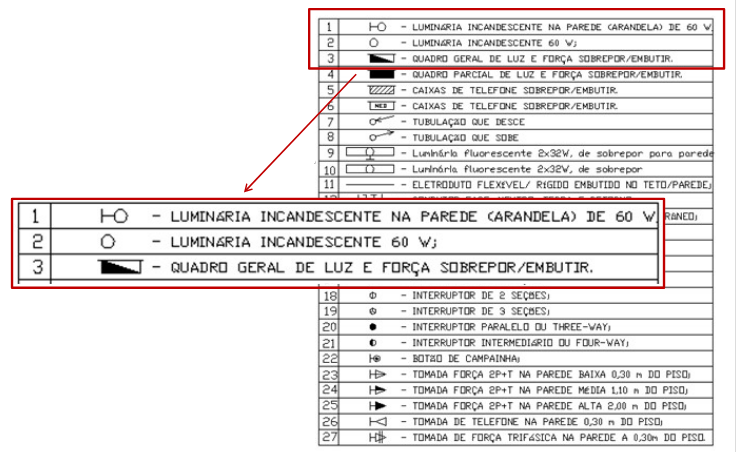
\includegraphics[scale=0.75]{Fig/Figura_ExemploLegenda.png} 
\caption{Exemplo de legenda}
\label{fig_ExemploLegenda}
\end{figure}

\hspace{1cm} São mostrados modelos deferentes de legendas a serem utilizadas em projetos A4 até A0 na Figura \ref{fig_ModelosLegendaA4ateA0}.

\begin{figure} [H] %[!h]
\centering
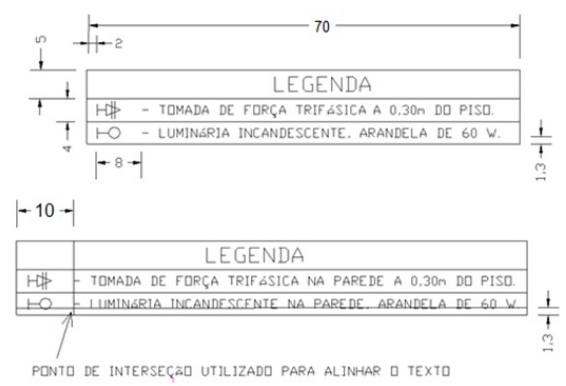
\includegraphics[scale=0.7]{Fig/Figura_ModelosDeLegendasA4ateA0.png} 
\caption{Modelos de legendas de projetos A4, A3, A2 e A0}
\label{fig_ModelosLegendaA4ateA0}
\end{figure}

\section{Lista de materias}

\hspace{1cm} A lista de materiais, como visto na Figura \ref{fig_ListaMateriais} é uma tabela contendo a descrição, unidade de venda e quantidade de materiais elétricos utilizados na obra.

\begin{figure} [H] %[!h]
\centering
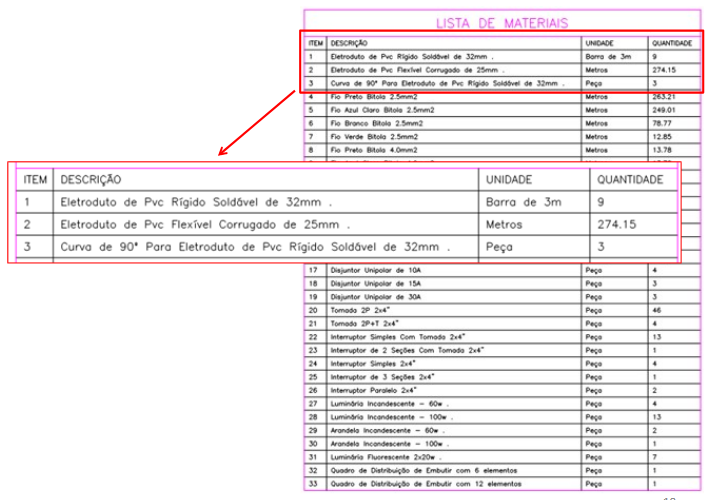
\includegraphics[scale=0.65]{Fig/Figura_ListaDeMateriais.png} 
\caption{Exemplo de lista de materiais}
\label{fig_ListaMateriais}
\end{figure}

\vspace{3.5cm}

\bibliography{references_correcao.bib}
\end{document}



